% ****** Start of file apssamp.tex ******
%
%   This file is part of the APS files in the REVTeX 4.2 distribution.
%   Version 4.2a of REVTeX, December 2014
%
%   Copyright (c) 2014 The American Physical Society.
%
%   See the REVTeX 4 README file for restrictions and more information.
%
% TeX'ing this file requires that you have AMS-LaTeX 2.0 installed
% as well as the rest of the prerequisites for REVTeX 4.2
%
% See the REVTeX 4 README file
% It also requires running BibTeX. The commands are as follows:
%
%  1)  latex apssamp.tex
%  2)  bibtex apssamp
%  3)  latex apssamp.tex
%  4)  latex apssamp.tex
%
\documentclass[superscriptaddress,unsortedaddress,
%runinaddress,
%frontmatterverbose, 
%preprint,
%preprintnumbers,
%nofootinbib,
%nobibnotes,
%bibnotes,
 amsmath,amssymb,
 aps,
%pra,
%prb,
%rmp,
%prstab,
%prstper,
%floatfix,
]{revtex4-2}

\usepackage{graphicx}% Include figure files
\usepackage{dcolumn}% Align table columns on decimal point
\usepackage{bm}% bold math
\usepackage{physics}
\usepackage{lipsum}
\usepackage{subfig}
% \usepackage{braket}

%\newcommand\abs[1]{\left|#1\right|}
%\newcommand\bra[1]{\left| #1 \right \rangle}
%\newcommand\ket[1]{\left \langle #1 \right |}

\begin{document}


\title{Predicting Solid State Qubit Candidates}

\author{Oliver Lerstøl Hebnes}
\affiliation{Department of Physics and Center for Computing in Science Education, University of Oslo, N-0316 Oslo, Norway}
\author{Marianne Etzelm\"uller Bathen}
\affiliation{Advanced Power Semiconductor Laboratory, ETH Zürich, 8092  Zürich,  Switzerland}
\affiliation{Department of Physics and Center for Materials Science and Nanotechnology, University of Oslo, N-0316 Oslo, Norway}
\author{Øyvind Sigmundson Schøyen}
\affiliation{Department of Physics and Center for Computing in Science Education, University of Oslo, N-0316 Oslo, Norway}
\author{Sebastian G. Winther-Larsen}
\affiliation{Department of Physics and Center for Computing in Science Education, University of Oslo, N-0316 Oslo, Norway}
\author{Morten Hjorth-Jensen}
\affiliation{Facility for Rare Ion Beams and Department of Physics and Astronomy, Michigan State University, East Lansing, MI 48824, USA}
\affiliation{Department of Physics and Center for Computing in Science Education, University of Oslo, N-0316 Oslo, Norway}
\author{Lasse Vines}
\affiliation{Department of Physics and Center for Materials Science and Nanotechnology, University of Oslo, N-0316 Oslo, Norway}

\begin{abstract}

Semiconductor materials provide a compelling platform for quantum
technology, and a vast amount of materials and their properties can be
found in high-throughput databases.  However, filtering among these
materials in order to find novel candidates for quantum technology is
a challenge. Therefore, we provide a framework for the automatic
discovery of promising solid-state material hosts using machine
learning methods.

%Main message 1: develop methodology for data mining and machine learning for materials properties 
We have developed data extraction tools for numerous material science
databases, and constructed over $4800$ physics-informed features for a
dataset consisting of more than $25000$ materials.  Furthermore, we
have developed and implemented three data mining approaches, termed
\textit{the Ferrenti approach}, \textit{the augmented Ferrenti
  approach} and \textit{the insightful approach} for defining three
distinct training sets for the supervised machine learning algorithms
logistic regression, decision tree, random forest and gradient boost
to be trained on.

% Main message 2: Use method to propose new materials that are promising quantum hosts 
We find a lack of consistent results for the Ferrenti approach and the
augmented Ferrenti approach due to an overly broad formulation of the
training set, whereas the restrictions set in the insightful approach
proved suitable. All models agreed on $214$ predicted candidates, with
examples such as ZnGeP$_2$, MgSe, CdS, BP, BC$_2$N, BP, Ge, GeC, InP,
and InAs. All approaches and all models agreed on a subset of $47$
eligible candidates of $8$ elemental, $29$ binary, and $10$ tertiary
compounds.

\end{abstract}

\pacs{02.70.Ss, 31.15.A-, 31.15.bw, 71.15.-m, 73.21.La}




\maketitle

%Submit to npj Computational Materials

%Marianne: I have now structured the paper according to other papers in this journal 
%I think we can make a supplementary material if we see that we need it, it is quite common for the journal 

\section*{Introduction}%Oliver and Morten and Marianne (semiconductor portion)
To sustain the digital world’s increasing computational demand, alternatives to the classical computer must be explored. The quantum computer, together with the complementary quantum technologies of sensing and communication, is becoming a frontrunner in the race for solutions. 
Discuss recent benchmarks for quantum computing \cite{Arute_2019}. 

Limitations of quantum computing and technology building blocks. Drawbacks of superconductors. Semiconductors are a promising platform. Example of NV center in diamond \cite{Doherty_2013}. 

%From thesis - rewrite 
Unfortunately, there are substantial challenges associated with the modern quantum platforms simultaneously as the selection of quantum platforms are slim. The majority of discoveries of potential quantum platforms have so far happened by serendipity, and there is an urgent need for new and better materials that can escalate the effort for a sustainable future. 

The fourth science paradigm introduces the potential of targeted search for promising material systems to act as qubit hosts. 
Herein, we provide a framework for the automatic discovery of promising solid-state material hosts using machine learning methods. 
Initial database building similar to Ferrenti et al \cite{Ferrenti2020}. 

\begin{figure}
    \centering
    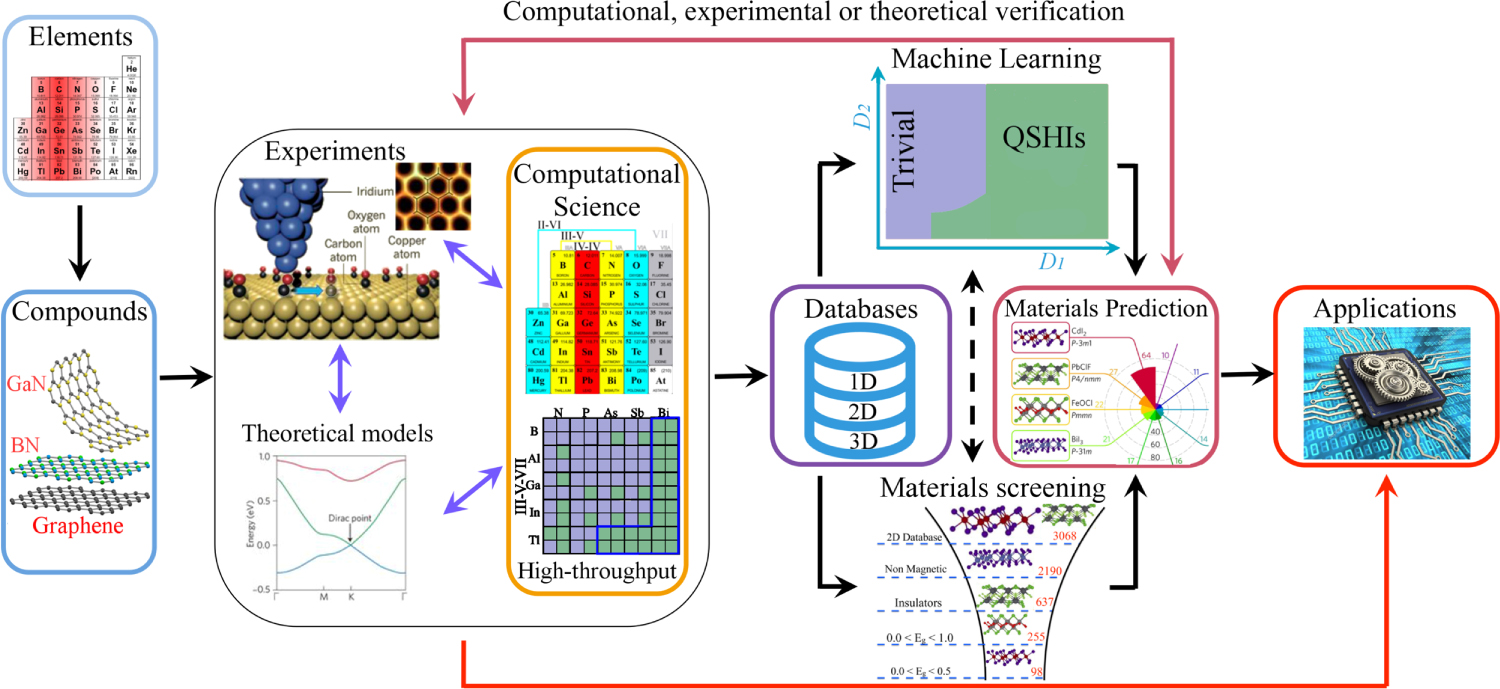
\includegraphics[width=\textwidth]{figures/ht-workflow.jpg}
    \caption{Placeholder for workflow. Morten: can you please add the other schematic figure we discussed as placeholder? Sebastian makes our own versions of these schematic figures (I can make some VESTA files with materials). }
    \label{fig:ht-workflow}
\end{figure}

\section*{Theoretical Background and Experimental Data} 
%Not all papers have a theory chapter, but since we are speaking to two quite different communities, it might be nice to include some basics. 
Quantum technologies, including sensing, communication and computing, 
are intriguing because of the new capabilities they offer. 
However, realization of large-scale fabrication for these techniques requires further technological development. 
The superconducting electronics platform that is currently employed for quantum computers necessitates millikelvin temperatures and may prove challenging to scale. 
Instead, recent developments have seen/heralded the rise of semiconductors as host materials for a variety of quantum devices. Much easier to combine with existing devices, and RT operation has been shown. 
However, the ideal host has yet to be identified, and the requirements for acting as a good host remain unclear. 
Different methods are needed. 

\subsection*{Semiconductors as a Quantum Host} %Marianne and Lasse 
The key feature when considering a quantum object for application is coherence, which is again tightly connected to the concept of coherence. 
For all applications, the basic requirement is a two-level quantum system which is quite isolated so the levels remain stable. 
Also need to control the qubit state via initialization, manipulation and read-out. 
Requirements \cite{DiVincenzo2000,Weber2010}: 
\begin{itemize}
    \item A scalable physical system with well-characterized qubits
    \item Reliable qubit initialization protocols 
    \item Need quantum gates to operate on qubits 
    \item Qubit state coherence time must exceed gate operation time 
    \item Need to read out qubit state after operation. 
\end{itemize}

%Discuss experimental data and the semiconductor platform. 
Semiconductors embody point defects that may trap charge carriers, causing deep energy levels to appear within the fundamental band gap. 
Importantly, such deep levels can trap carriers in localized states that are essentially isolated from the surroundings, making them suitable for QT. 
A prime example is the nitrogen-vacancy center in diamond, which has been proposed 
as a contender for both qubit, sensing and communication applications \cite{Doherty_2013}. 
The NV center is a room temperature single-photon source emitting in the visible portion of the spectrum, exhibiting entangled photons that have been separated by ... km []. 
Moreover, the NV center in its negative charge state traps an electron in a localized and high-spin $S=1$ state that can be coherently controlled and with RT spin coherence of 1 ms []. 
Qubit operations and entanglement have been demonstrated []. 
However, emission wavelength is not ideally compatible with fiber optic technology (need telecom range), spin coherence is good but could be better, and sensing is good. 

\begin{table}[t]
    \centering
    \begin{tabular}{c|c|c|c}
    Material & Band gap (eV) & Defect candidates & Reference \\
    \hline
    Diamond  & $5.5$  & N$_\mathrm{C}V_\mathrm{C}$, Si$_\mathrm{C}V_\mathrm{C}$, Ge$_\mathrm{C}V_\mathrm{C}$ & \cite{Balasubramanian_2009,Rogers_2014,Bhaskar_2018} \\  
    4H-SiC & $3.3$ & $V_\mathrm{Si}$, $V_\mathrm{Si}V_\mathrm{C}$, C$_\mathrm{Si}V_\mathrm{C}$, N$_\mathrm{C}V_\mathrm{Si}$ & \cite{Widmann2014,Christle_2015,Castelletto_2014,Zargaleh_2018} \\ 
    Si & $1.1$ & P, G, unidentified & \cite{Muhonen_2014,Durand_2020,Redjem2020} \\ 
    (2D) \textit{h}-BN & $6.0$ & Unidentified defects & \cite{Tran_2016,Tran_2016b,Hayee_2020} \\ 
    ZnO & $3.4$ & Unidentified defects & \cite{Morfa2012} \\ 
    ZnS & $3.6$ (zincblende) & Unidentified defects & \cite{Stewart2019} \\ 
    GaAs & $1.4$ & Quantum dots & \cite{Bluhm2010} \\ 
    GaN & $3.4$ & Quantum dots, unidentified defects & \cite{Roux2017,Berhane2018} \\
    AlN & $6.0$ & Unidentified defects & \cite{Xue2020}\\
    \end{tabular}
    \caption{Overview of materials and defects that have been demonstrated to exhibit QT-compatible characteristics such as single-photon emission and coherent spin manipulation.}
    \label{tab:qt-materials}
\end{table}

 ZnS [74], GaAs [75],
GaN [76, 77 , 80] and AlN [78, 79],  [81]. 

%QT requirements. 
%What parameters are we looking for? 
Table \ref{tab:qt-materials} contains an overview of known semiconductor materials with demonstrated quantum compatible characteristics. 
Not all defects are identified, and challenges due 
to the specific materials complicate the implementation of defects for QT. 
There are some common denominators for the materials: 
\begin{itemize}
    \item Wide band gap to facilitate localized deep levels (physical)
    \item Low spin orbit coupling to extend spin coherence times (physical) 
    \item Low el-phonon coupling for sharp ZPLs (physical) 
    \item Availability as high-quality, bulk, or thin-film single crystals (practical)
    \item Constituent elements with naturally occurring isotopes of zero nuclear spin (practical). 
\end{itemize}
Note the division between physical and practical requirements in the list above. 
The physical ones refer to some fundamental aspect of the material that permits specific properties to manifest, while practical refers to some more external influence that provides more easy measurement and detection of said properties. 
It is the former that we are interested in. 

Different defect and material types may suit different needs. 
Therefore, we need a bigger bank of candidates. 
Also, we do not fully understand exactly what constitutes a good quantum host material. 
So far, detection of QT compatibility has been slow, as a signal is detected and then identified in a specific material. 
We are looking for a top-down approach to instead predict promising materials, and guide experiments. 
For this, we first need a large dataset. 

\subsection*{Density Functional Theory Output} %Marianne 
Density functional theory has been exceptionally successful in predicting solid-state material properties 
such as 

Data formats, limitations etc.  

Density functional theory is a versatile and powerful theoretical approach, enabling targeted study of semiconductor materials with many atoms. 
Proven successful for material properties such as thermal stability, lattice parameters and band gap. 



\subsection*{Material Informatics} %Øyvind (Oliver)    
%Data mining, screening 

\subsection*{Machine Learning} % Morten 

\section*{Results}
Includes discussion of results.  

\subsection*{Information Flow}  %Sebastian/Oyvind (Marianne) 
Includes results from data mining and description of the three approaches. 
%MEB: Since Methods are at the end, I propose to put part of this discussion in the Results section. 
%This is because it is an important result of the work, and also because it is important to understand the rest of the paper 

\subsection*{Optimization of Machine Learning Models} %Morten (Oliver input in round 2)

\subsection*{Predicting Novel Material Hosts for Quantum Technology} %Oyvind (Oliver input in round 2) 
\subsubsection*{The Ferrenti approach} 
\subsubsection*{The augmented Ferrenti approach}
\subsubsection*{The insightful approach}
\subsubsection*{Comparing the approaches}

\section*{Discussion} % All - last thing we write  
Shorter section, includes summary, concluding remarks and is quite heavy on outlook.  

\section*{Methods}
%Methodology comes after concluding remarks, and is structured into subsections 

\subsection*{Databases} %Oliver and Øyvind 
%Materials project, AFLOW, Open Quantum, JARVIS 
Mining.  

\subsection*{Material Informatics} %Oliver and Øyvind 
Screening and workflow and approaches.  

\subsection*{Machine Learning} %Sebastian/Morten   
Insight gaining. 

\section*{Data availability} 
%We can put something else, standard text 
The data that support the plots within this paper and other findings of this study are
available from the corresponding authors upon reasonable request.

\section*{Code availability} 
The codes developed in this study are available from the authors upon reasonable
request.

\bibliography{apssamp}% Produces the bibliography via BibTeX.

\begin{acknowledgments}

The work of MHJ is supported by the U.S. Department of Energy,
Office of Science, office of Nuclear Physics under grant
No. DE-SC0021152 and U.S. National Science Foundation Grants
No. PHY-1404159 and PHY-2013047. 
The work of MEB and LV was supported by the Research Council of Norway and the University of Oslo through the frontier research project FUNDAMeNT (no. 251131, FriPro ToppForsk-program). 
%Some of the computations were performed on resources provided by UNINETT Sigma2 - the National Infrastructure for High Performance Computing and Data Storage in Norway.  
The work of MEB was supported by an ETH Zurich Postdoctoral Fellowship. 

\end{acknowledgments}

\section*{Author contributions} 
%Copied in from another paper 
S.-M.J. conceived the idea and developed the simulation model. T.H.L. performed
computer simulation. S.Y.B. and S.D.H. fabricated devices. D.-W.S., S.L., H.W.C. and
J.-W.J. supported measurement of device performances. Y.-H.S. and X.-B.F.
synthesised QD materials. S.Z. and J.Y. supported experiments. C.S. and Y.K.
supported computer simulation. L.G.O. and G.A. supported data analysis. J.M.K.
guided this work. S.-M.J., T.H.L. and S.Y.B. contributed equally. 
All the authors contributed to the preparation of the manuscript.

\section*{Competing interests}
The authors declare no competing interests.


\end{document}

